\chapter{Justificacion}

Aunque en México existen compañías netamente mexicanas que laboran con Sistemas Integrados, como la compañía de teléfonos celulares Zonda Telecom [8] no es un mercado muy explotado como en otros países de primer mundo, se manufacturan muchos de estos sistemas, pero sería una gran adelanto y una gran ventaja para nuestro país que muchos más ingenieros mexicanos tuvieran un acceso a seguir desarrollándolos en el ramo de sus elección, ya sea en instrumentos musicales digitales, aire acondicionado, calculadoras, y que mejor que en aviónica y equipos médicos.\medskip

Diseños mexicanos explotando este mercado le generaría a México un fuerte ingreso de capital, por las ventas que estos productos, empleos para realizarlos, y por supuesto prestigio de que en este país se hacen productos de calidad, innovadores y seguros.\medskip

Por eso nuestra tentativa solución a este mercado inexplorado el presente proyecto de Trabajo Terminal que pretende atacar el problema con los siguientes puntos a favor. \medskip

{\em Originalidad del trabajo}. Como ya lo hemos mencionado antes, esta “consola” es un producto que aunque se han desarrollado algunas versiones parecidas, no de la forma en que la tenemos planeada, hablando del software, pues usaremos conceptos nuevos en su desarrollo.\medskip

{\em Vinculación con los usuarios potenciales}. Los beneficios serían principalmente para los estudiantes de ingeniería que quieran investigar de este tema, y quieran tener algo como base para hacer sus propios diseños.\medskip

{\em Complejidad}. Nuestros conocimientos en Sistemas Operativos, Electrónica Analógica, Circuitos Eléctricos, pero más nuestras ganas de investigar, no han llevado a buscar la forma de realizar este proyecto con los mejores componentes, novedosos pero necesarios, sin desperdiciar utilidad de los mismos, también nos han ayudado a ver los antiguos modelos de productos parecidos al de nosotros, y pensar en una mejoría, tanto en costo, como en rentabilidad, calidad y apariencia.\medskip

{\em Tecnología}. Queremos principalmente con este proyecto aprender como son los sistemas integrados, saber en que los podemos usar, que ramos de la industria se pueden mejorar con la aplicación de ellos, todo este conocimiento adquirido bien empleado traería consigo un gran avance en la tecnología del país.\medskip

Se han evaluado varias tecnolog\'ias que se pueden utilizar en sistemas embedidos, y hemos optado por una basados en los requerimientos que tenemos.

Las tecnolog\'ias mas interesantes han sido las siguientes:

\begin{itemize}
\item PIC
\item AVR
\item Blackfin
\item MIPS
\item ARM
\end{itemize}

La tecnolog\'ia PIC de Microchip es una de las m\'as usadas en nuestro pa\'is, es bastante buena en caso de que se deseen hacer sistemas de bajo consumo de un tama\~no muy peque\~no, sin embargo es dif\'icil utilizarla en aplicaci\'ones que demandem m\'as capacidad.

Las tecnolog\'ia AVR de ATMEL tiene caracter\'isticas muy similares a las del PIC, lo que dificulta trabajarla en aplicaciones de mas alta capacidad.

Las otras arquitecturas revisadas permiten el uso externo de una memoria RAM, lo cual facilita utilizarlas en aplicaciones mas demandantes.

Blackfin es un microprocesador libre, el fabricante da toda la documentaci\'on e incluso acepta mejoras a la arquitectura. Es utilizado sobre todo en equipo de redes de bajo costo, como routers, switches, etc. Sin embargo no est\'a pensado para dispositivos m\'oviles por lo que no es de bajo consumo. 

La tecnolog\'ia MIPS es un est\'andar que define una empresa, y los fabricantes pueden implementarlo. Microchip tiene una implementaci\'on sin embargo no tiene acceso a memoria RAM, otros fabricantes como Samsung tambi\'en tienen sus microprocesadores pero es dif\'icil tener acceso a ellos.

Por \'ultimo tenemos la tecnolog\'ia ARM, al igual que MIPS es tan s\'olo una especificaci\'on y hay varios fabricantes que la han implementado como: Intel, ATMEL, Samsung, etc. Lo interesante de esta arquitectura es que hay desde microcontroladores con capacidades similares a un PIC, hasta microcontroladores capaces de controlar un iPhone, y como la arquitectura es la misma, tenemos compatibilidad binaria entre \'ambos, es por ello que la arquitectura ARM es una de las m\'as usadas actualmente.

Las tablas mostradas a continuación demuestran que el uso de tecnologias ARM esta a la alza y se esta convirtiendo en la opción a futuro para grandes desarrolladores de nuevas tecnolog\'ias a nivel mundial.

\begin{figure}[H]
\centering
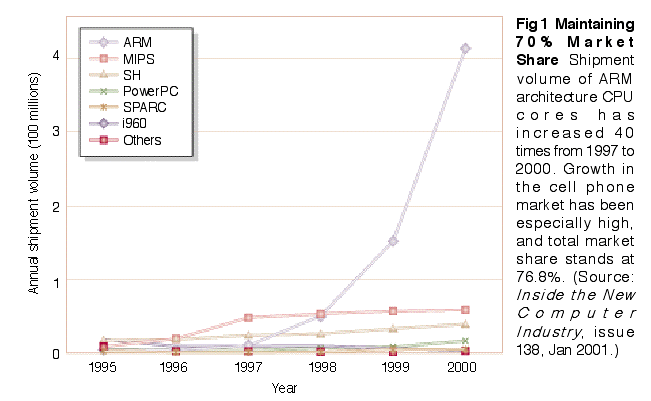
\includegraphics[scale=0.4]{tablaarm1}
\caption{Tabla 1}\label{fig:tablaarm1}
\end{figure}
{\em http://www.design\-reuse.com/news\_img/20090430\_microprocessor\-market\-forecast.gif}

\begin{figure}[H]
\centering
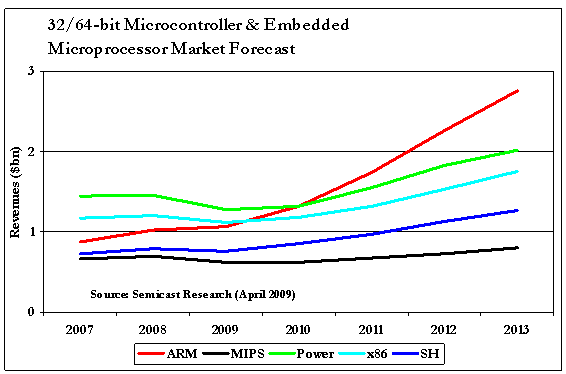
\includegraphics[scale=0.4]{tablaarm2}
\caption{Tabla 2}\label{fig:tablaarm2}
\end{figure}
{\em http://www.design\-reuse.com/news\_img/20090430\_microprocessor\-market\-forecast.gif}

